\section{대전시 스마트 모빌리티 통합 플랫폼}

\subsection{서비스 개요}
대전시 스마트 모빌리티 플랫폼은 지하철, 타슈(공공자전거), 버스를 통합한 멀티모달 경로 탐색 서비스입니다. 사용자 위치 기반 실시간 경로 안내와 교통수단별 최적 환승 정보를 제공합니다.

\begin{figure}[h]
    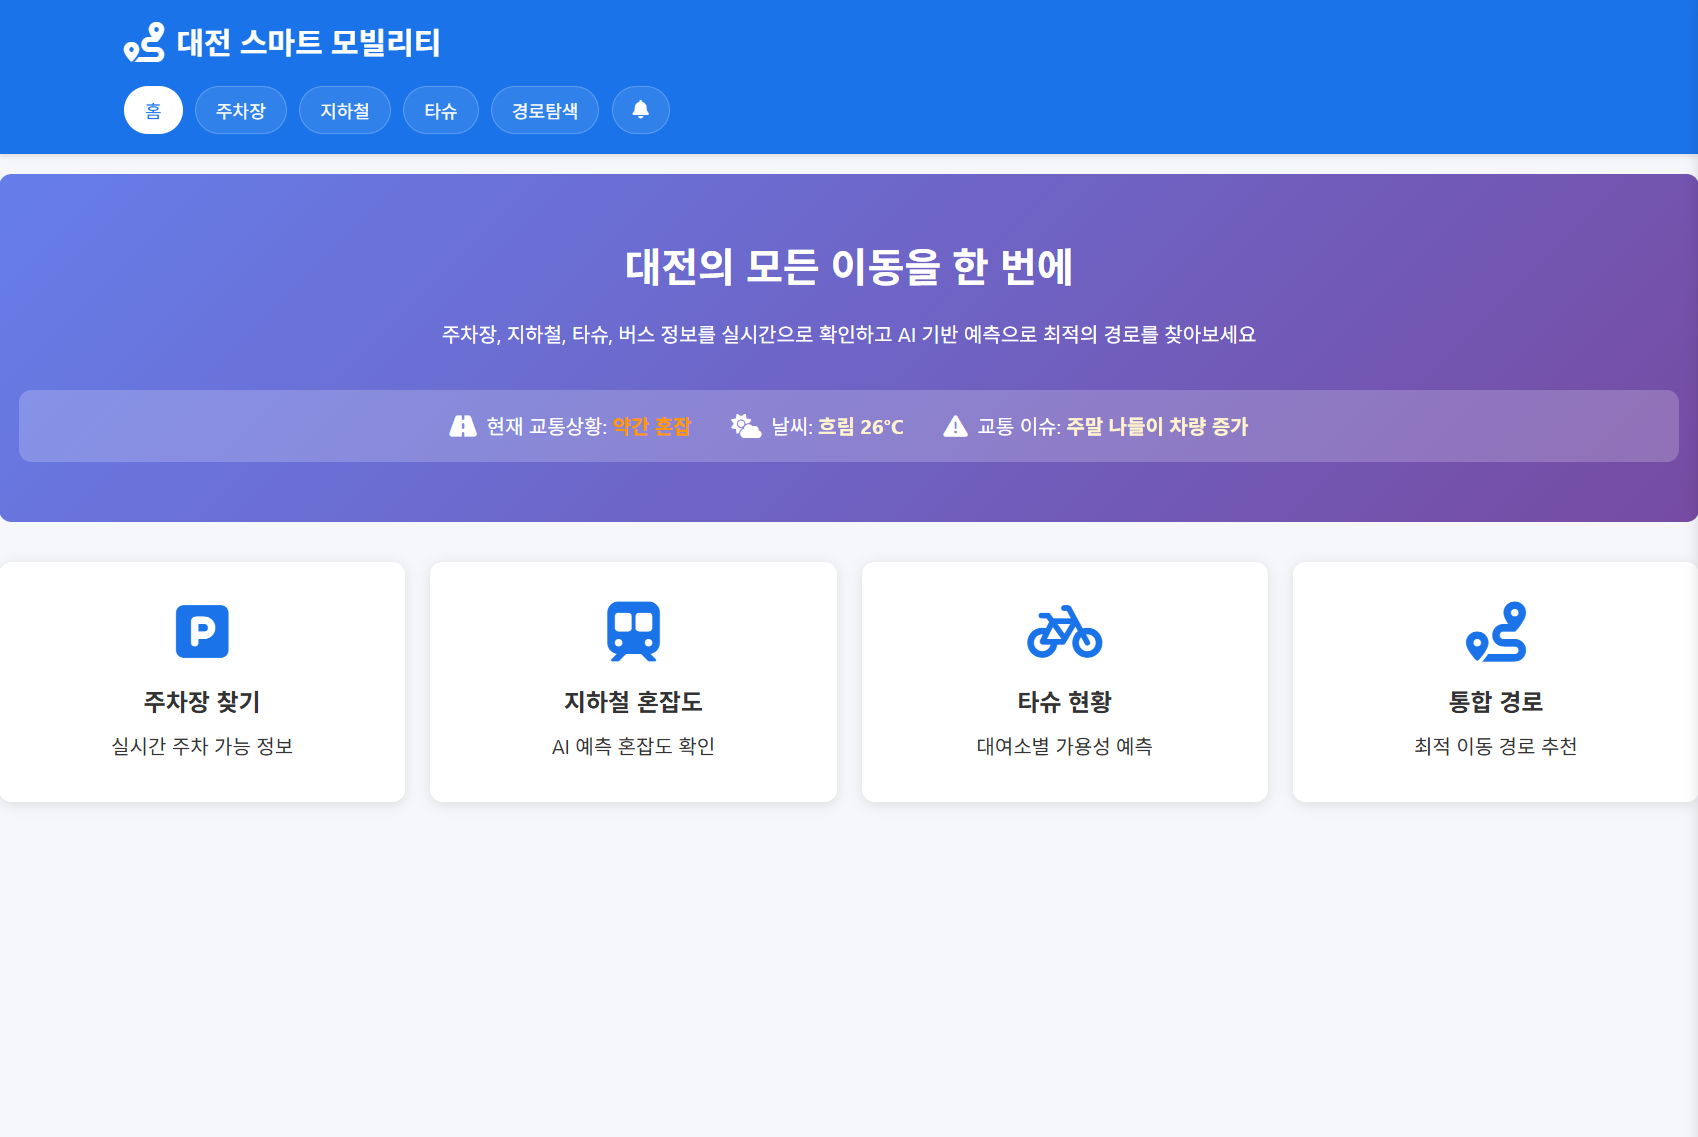
\includegraphics[width=\columnwidth]{2/daejeon-1.png}
    \caption{대전 스마트 모빌리티 메인 인터페이스 - 통합 교통 선택 화면}
    \label{fig:main_interface}
\end{figure}

\subsection{시스템 아키텍처}

\subsubsection{데이터 통합 레이어}
대전시 공공데이터 포털의 실시간 API를 활용하여 교통 정보를 수집합니다. 지하철 1호선 21개 역사 정보, 타슈 대여소 97개소 실시간 대여 현황, 주요 버스 노선 및 정류장 데이터를 통합 관리합니다.

\subsubsection{그래프 기반 경로 탐색}
교통 네트워크를 노드-엣지 그래프로 모델링하여 Dijkstra 알고리즘 기반 최단 경로를 산출합니다. 각 교통수단의 이동 속도와 환승 시간을 가중치로 적용하여 실시간 최적 경로를 제공합니다.

\begin{figure}[h]
    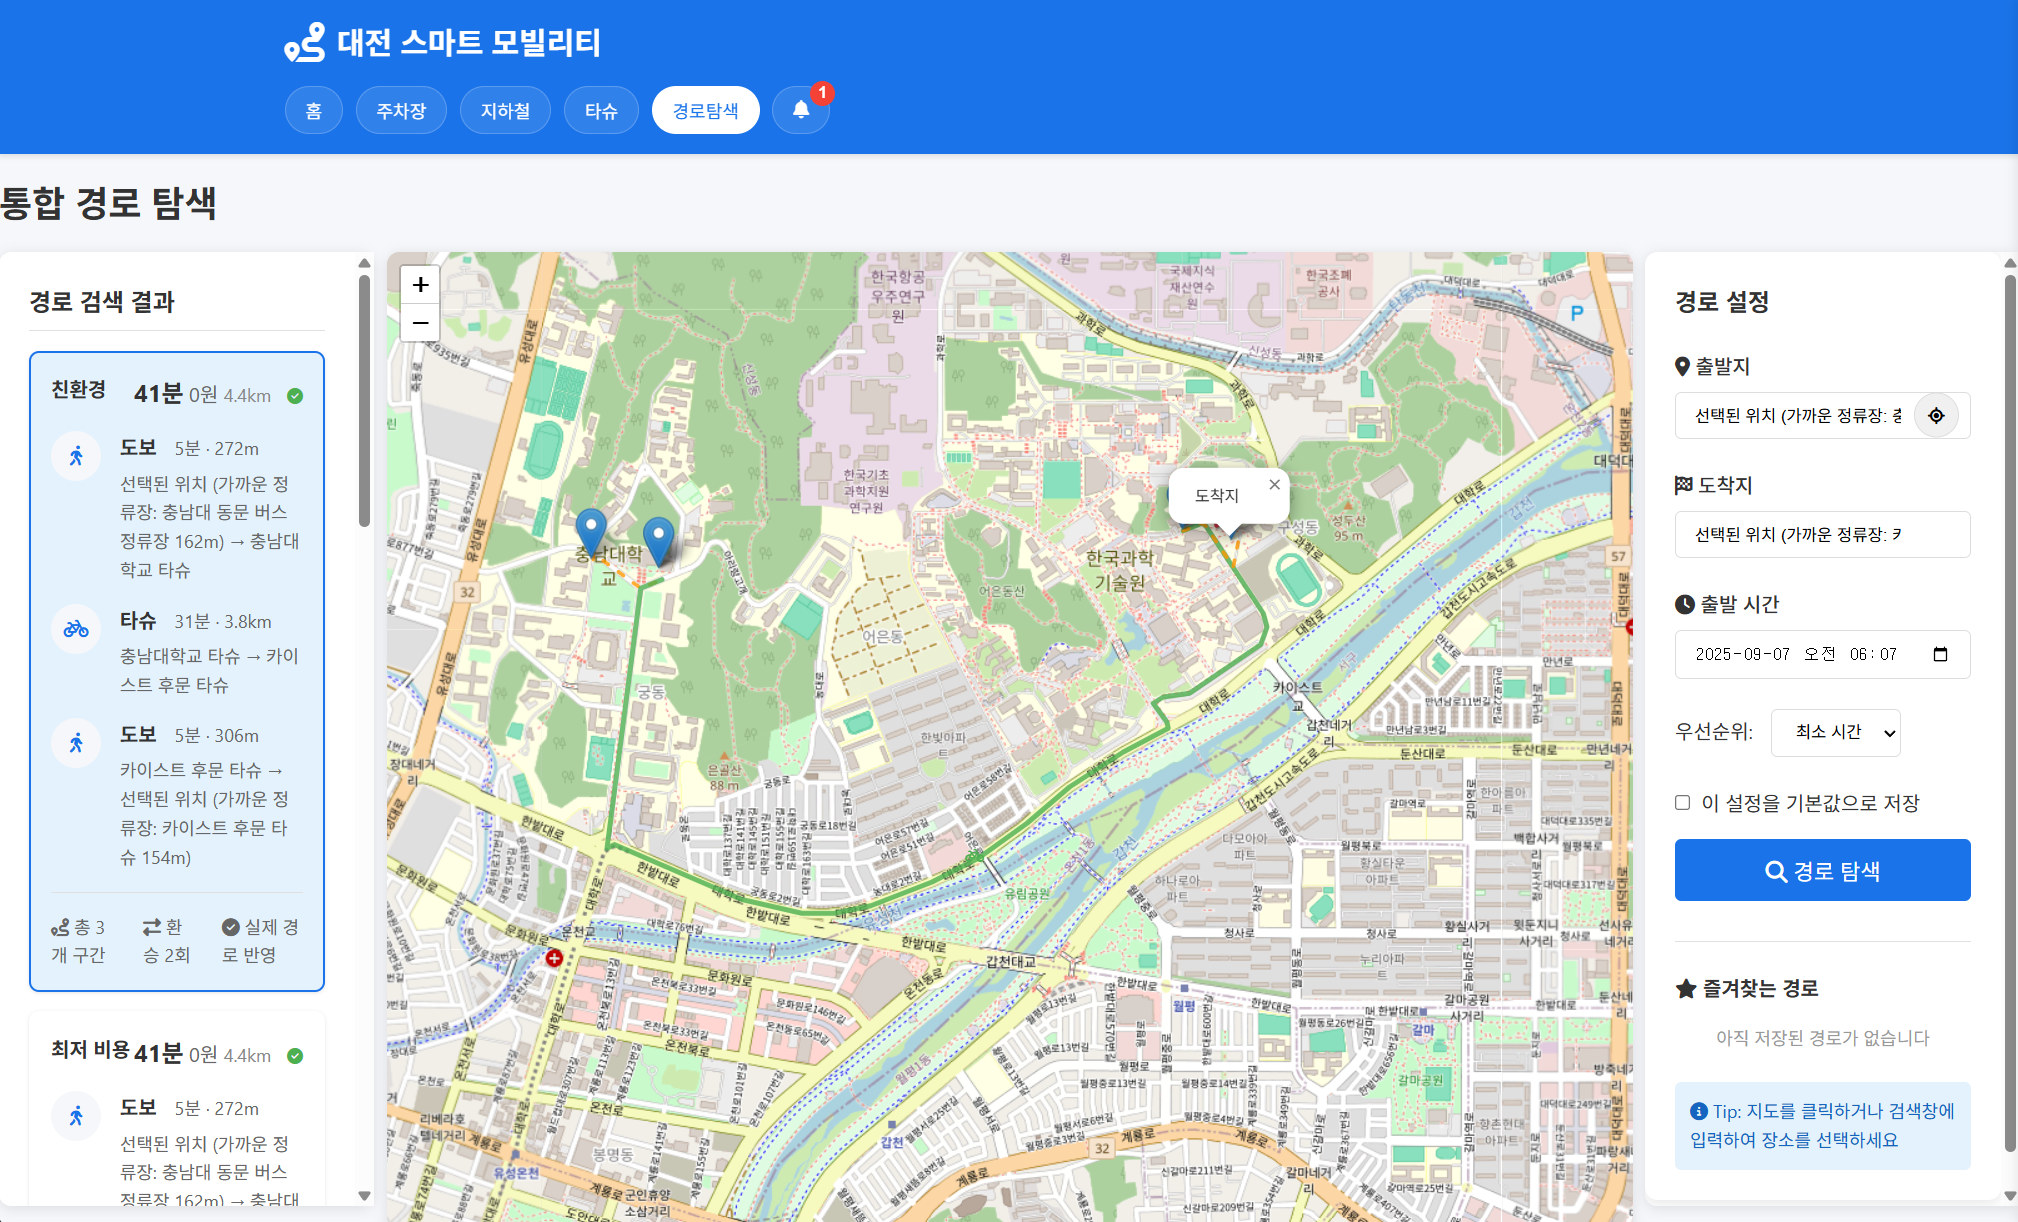
\includegraphics[width=\columnwidth]{2/daejeon-2.png}
    \caption{지도 기반 경로 탐색 - 출발지와 도착지 선택 인터페이스}
    \label{fig:route_selection}
\end{figure}

\subsection{핵심 기능 구현}

\subsubsection{실시간 경로 계산}
OSRM (Open Source Routing Machine) API를 활용하여 실제 도로 기반 경로를 계산합니다. 도보, 자전거, 대중교통 각각의 이동 시간을 정확히 산출하여 신뢰성 있는 경로 정보를 제공합니다.

\begin{verbatim}
class IntegratedTransportGraph {
    findMultimodalRoute(start, end, preference) {
        // Create virtual node and connect to nearby transport nodes
        const virtualStart = this.createVirtualNode(start);
        const nearestNodes = this.findNearestNodes(start, 0.8);
        
        // Find optimal route using Dijkstra algorithm
        const routes = this.dijkstra(virtualStart, end);
        
        // Recalculate with actual road paths
        return this.recalculateWithRealPaths(routes);
    }
    
    calculateDistance(lat1, lng1, lat2, lng2) {
        // Apply Haversine formula
        const R = 6371; // Earth radius (km)
        const roadDistanceFactor = 1.5; // Road detour factor
        return straightDistance * roadDistanceFactor;
    }
}
\end{verbatim}

\subsubsection{교통수단별 속도 설정}
실제 도시 환경을 반영한 현실적인 이동 속도를 적용합니다. 도보 5km/h, 타슈 25km/h, 버스 40km/h, 지하철 60km/h로 설정하여 정확한 소요 시간을 계산합니다.

\begin{figure}[h]
    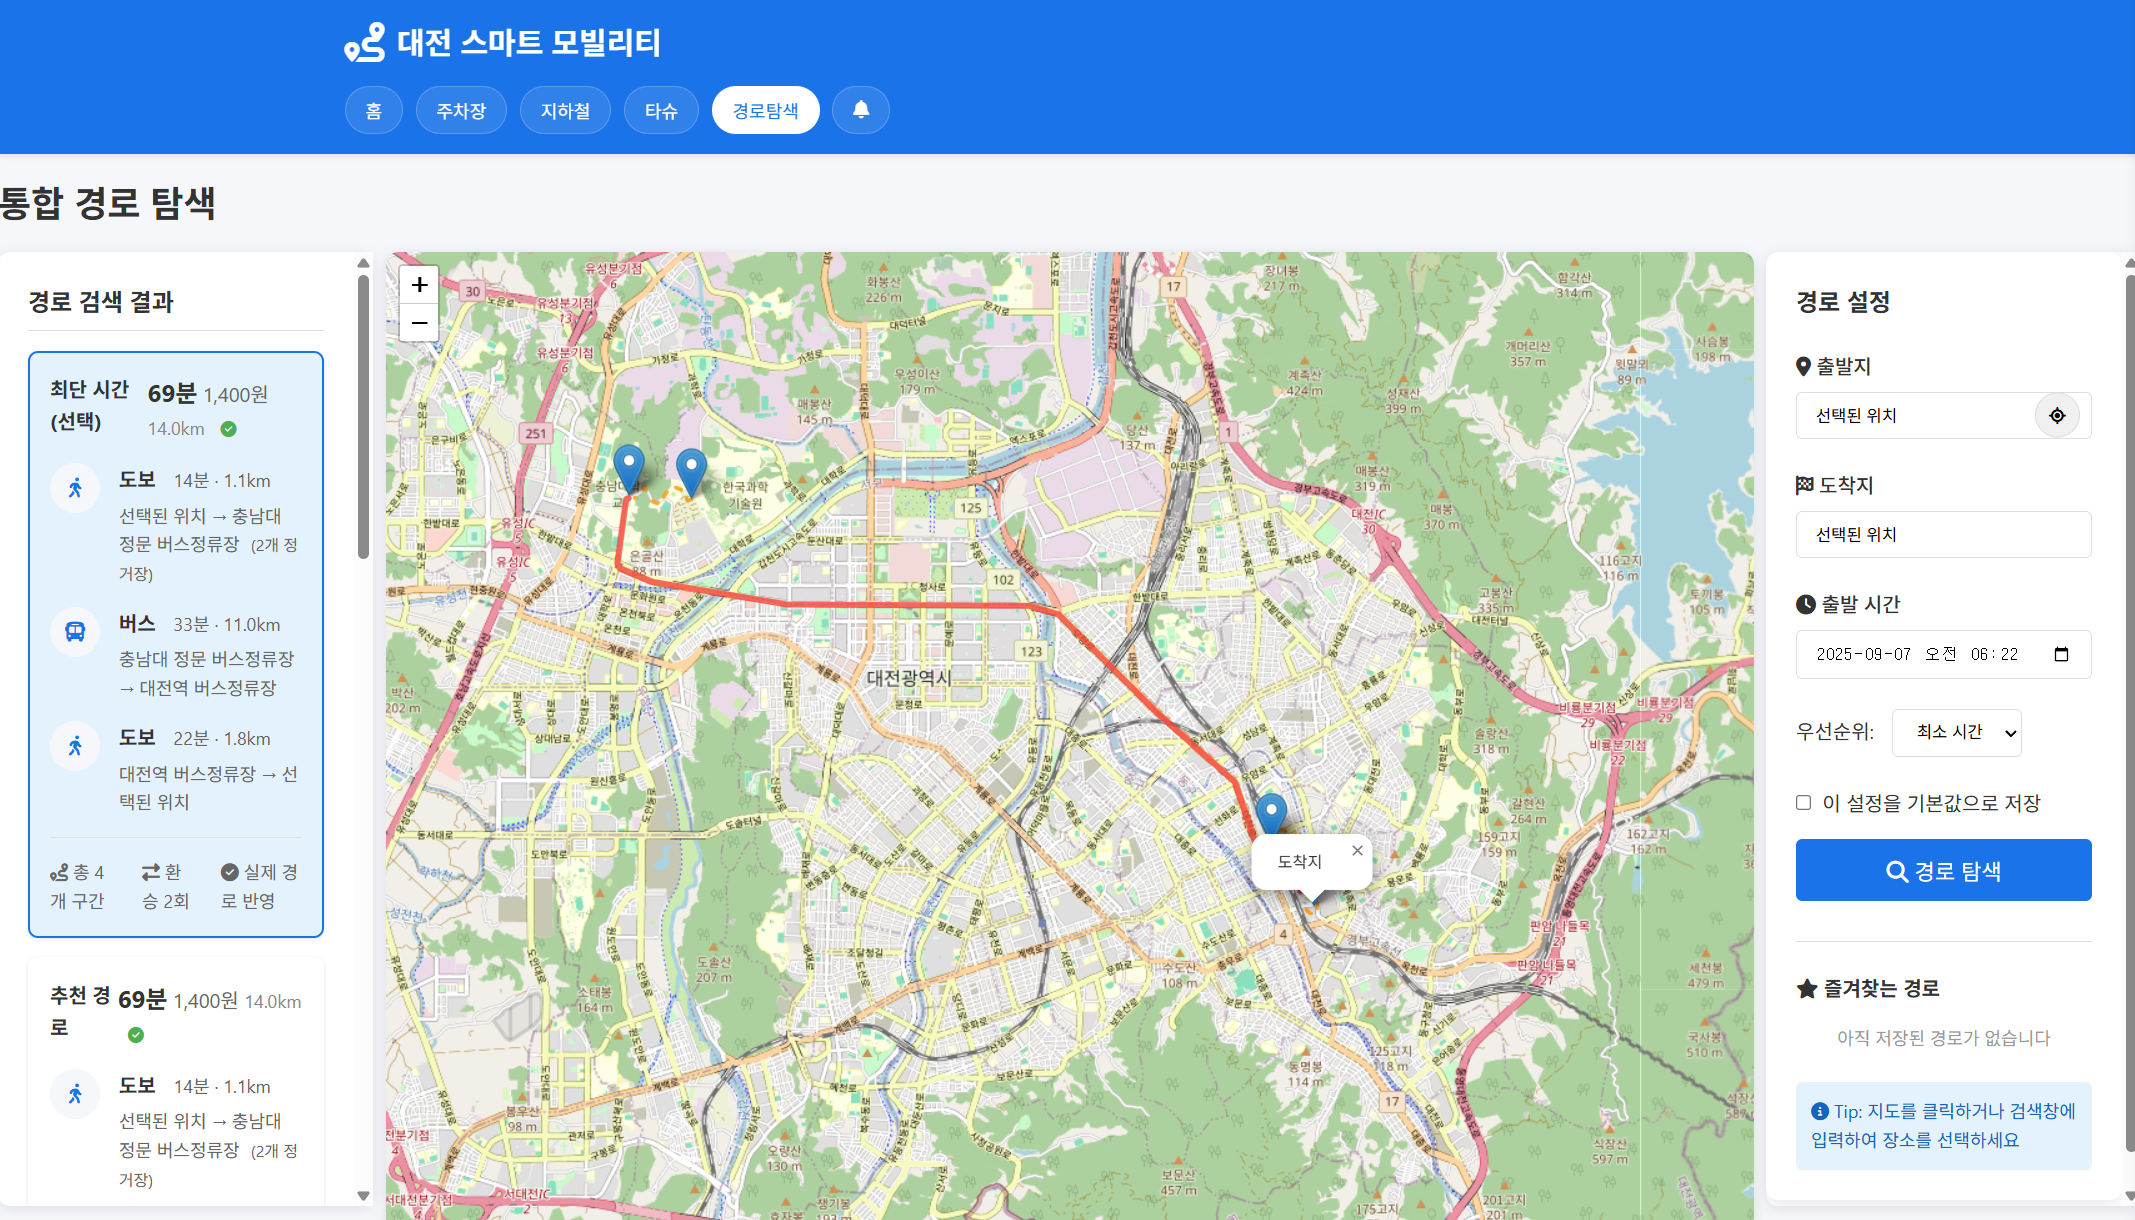
\includegraphics[width=\columnwidth]{2/daejeon-3.png}
    \caption{멀티모달 경로 결과 - 지하철과 도보를 결합한 최적 경로 표시}
    \label{fig:multimodal_route}
\end{figure}

\subsection{사용자 인터페이스}

\subsubsection{지도 기반 인터랙션}
Leaflet.js 기반 대화형 지도를 구현하여 직관적인 경로 선택이 가능합니다. 우클릭 컨텍스트 메뉴로 출발지와 도착지를 손쉽게 지정할 수 있으며, 실시간으로 경로가 지도상에 시각화됩니다.

\subsubsection{경로 옵션 비교}
복수의 경로 옵션을 제시하여 사용자가 상황에 맞는 최적 경로를 선택할 수 있습니다. 각 경로별 총 소요 시간, 이동 거리, 환승 횟수, 교통수단별 구간 정보를 명확히 표시합니다.

\begin{figure}[h]
    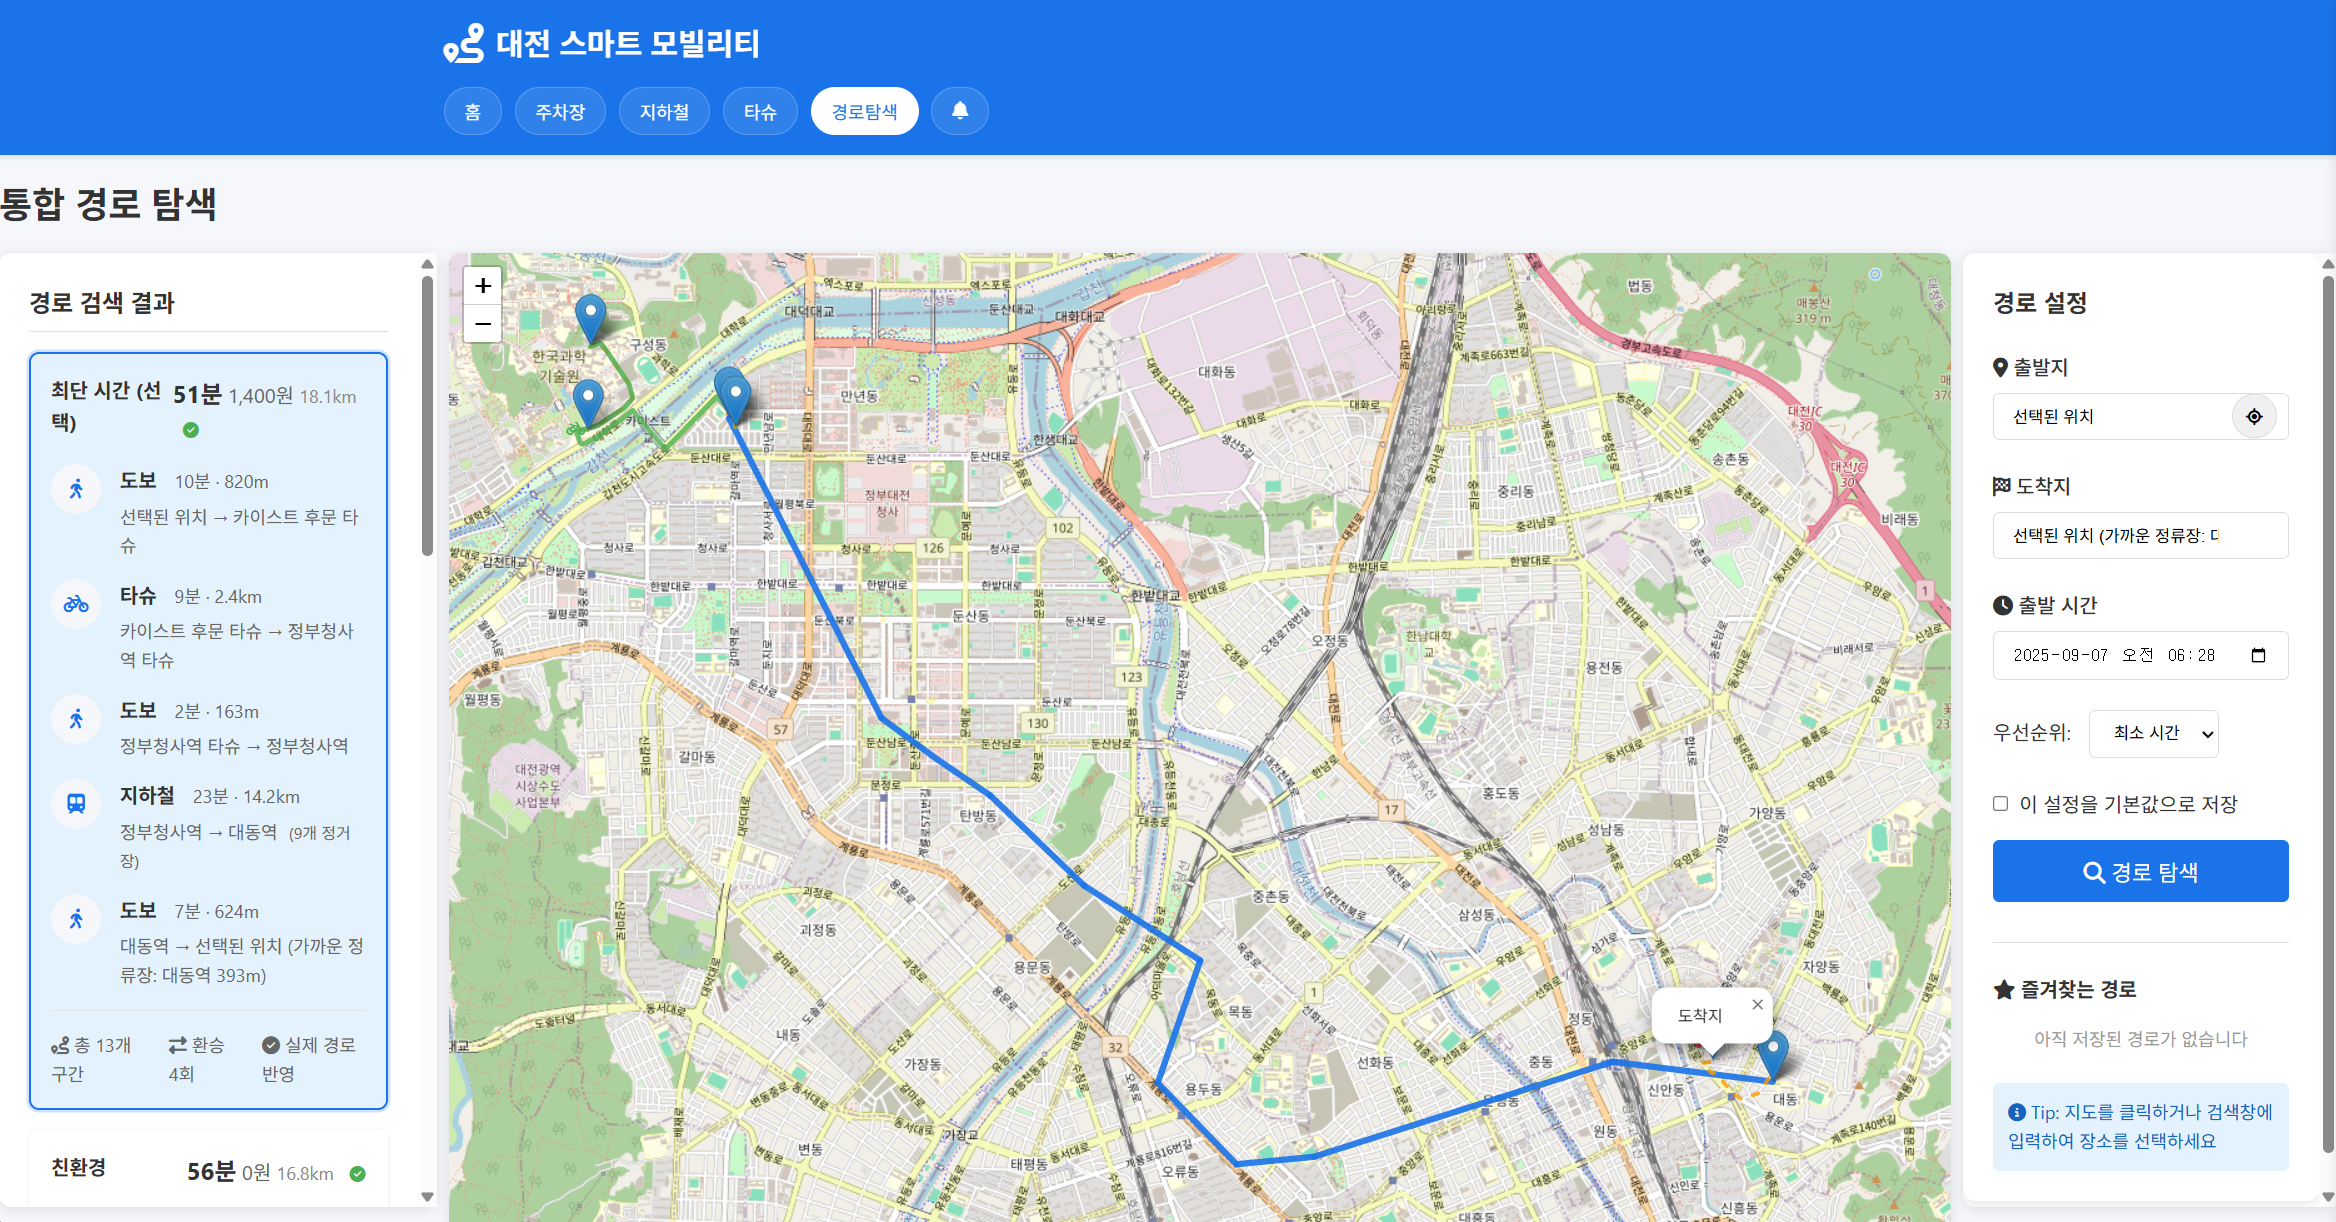
\includegraphics[width=\columnwidth]{2/daejeon-4.png}
    \caption{경로 상세 정보 - 구간별 교통수단과 소요 시간 표시}
    \label{fig:route_details}
\end{figure}

\subsection{기술적 특징}

\subsubsection{캐싱 전략}
반복적인 경로 요청에 대한 응답 속도 향상을 위해 LRU (Least Recently Used) 캐시를 구현했습니다. 15분간 동일 경로 요청 시 캐시된 데이터를 활용하여 서버 부하를 감소시킵니다.

\subsubsection{반응형 디자인}
CSS Grid와 Flexbox를 활용한 반응형 레이아웃으로 다양한 디바이스에서 최적화된 사용자 경험을 제공합니다. 모바일 환경에서도 지도와 경로 정보를 효과적으로 표시합니다.

\subsection{성과 및 기대효과}
본 플랫폼은 대전시민의 대중교통 이용 편의성을 크게 향상시킵니다. 실시간 교통 정보와 최적 경로 제공으로 이동 시간 단축과 대중교통 이용률 증가에 기여합니다. 특히 타슈와 대중교통의 연계 활용도를 높여 친환경 교통수단 이용을 촉진합니다.

향후 실시간 버스 도착 정보, 지하철 혼잡도, 날씨 기반 경로 추천 등의 기능을 추가하여 더욱 스마트한 도시 교통 플랫폼으로 발전시킬 계획입니다.